% !TEX root = ../tutorials.tex
\chapter{Advection Diffusion Reaction (ADR) Solver}
\label{ADR}

\section*{\Large Introduction}
Welcome to the Advection Diffusion Reaction (ADR) Solver tutorial for the Nektar++ library.
This tutorial is intended to show the main features of the ADR solver in a simple and user-friendly 
format. If you do not have already downloaded and installed Nektar++, please do so by visiting 
\href{http://www.nektar.info}{nektar.info}, where you can also find the user-guide with the instructions 
to install the library. This tutorial requires the pre- and post-processing tools and the ADR 
solver within Nektar++ and the open-source mesh generator \href{http://geuz.org/gmsh/}{Gmsh} 
and the visualisation tool \href{http://www.paraview.org}{Paraview}. If the links to Gmsh and Paraview 
are broken it should be sufficient to search for them in any web search engine.  


\subsubsection*{Goals}
After the completion of this tutorial, the user will be familiar with:
\vspace{-0.5cm}
\begin{itemize}
\item the generation of a simple mesh in Gmsh and its conversion into a Nektar++-compatible format.
\item the visualisation of the Jacobian distribution across the mesh in Paraview.
\item the setup of the initial and boundary conditions, the parameters and the solver settings.
\item running a simulation with the ADR solver.
\item the post-processing of the data and the visualisation of the results in Paraview.
\end{itemize}

\subsubsection*{Resources}
The files necessary to run this tutorial are included in ??.  
Specifically, two files with extension \textsf{.xml} are needed as input for Nektar++: 
\vspace{-0.5cm}
\begin{itemize}
\item a file containing the mesh: \inlsh{ADR\_mesh.xml};
\item a configuration file with the simulation settings \inlsh{ADR\_conditions\_aligned.xml}.
\end{itemize}

In the same folder it is possible to find also the following additional material:
\vspace{-0.5cm}
\begin{itemize}
\item a Gmsh file to generate the mesh, \inltt{ADR\_mesh.geo};
\item a .msh file containing the mesh in Gmsh format, \inltt{ADR\_mesh.msh};
\item a .xml file containing the mesh in Nektar++ format without the edges aligned 
for the periodic boundary conditions (see section \ref{adr-pre}), \inltt{ADR\_mesh.xml};
\item the 11 output .chk binary files generated by running the simulation, \inltt{ADR\_mesh\_aligned\_i.chk};
\item the 11 output files converted in a Paraview readable format (.vtu),  \inltt{ADR\_mesh\_aligned\_i.vtu};
\item the output .fld binary file generated at the last time-step of the simulation, \inltt{ADR\_mesh\_aligned.fld}.
\item a bash script to automatically convert the 11 .chk files into .vtu files, \inltt{convert.sh}
\end{itemize}

\begin{center}
Now that you are ready, lets' start!
\end{center}

\section{Background}
The ADR solver can solve various problems, including the unsteady advection, unsteady diffusion, 
unsteady advection diffusion equation, etc. For a more detailed description of this solver, please 
refer to the User-Guide. 

In this tutorial we focus on the unsteady advection equation
\begin{equation}
\dfrac{\partial u}{\partial t} + \mathbf{V}\cdot\nabla u = 0,
\label{eq:advection}
\end{equation}
where $u$ is the independent variable and $\mathbf{V} = [\text{V}_{x}\; \text{V}_{y}\; \text{V}_{z}]$ 
is the advection velocity. The unsteady advection equation can be solved in one, two and three spatial 
dimensions. We will here consider a two-dimensional problem, so that $\mathbf{V} = [\text{V}_{x}\; \text{V}_{y}]$.

\section{Problem description}
The problem we want to run consists of a two-dimensional Gaussian function travelling in the $x$-direction
at a constant advection velocity. In order to model this problem we create a computational domain also 
referred to as mesh or grid (see section \ref{adr-pre}) on which we apply a two-dimensional Gaussian 
function as initial condition and periodic boundary conditions at the mesh boundaries
%
\begin{equation}
\begin{array}{l}
\dfrac{\partial u}{\partial t} + \text{V}_{x}\dfrac{\partial u}{\partial x} + \text{V}_{y}\dfrac{\partial u}{\partial y} = 0,\\[1em]
u(x,y;\;t=0) = \sin(\kappa x) \cos(\kappa y),\\[1em]
u(x_{b} = [-1, 1],y_{b};\;t) = \text{periodic},\\[1em]
u(x_{b},y_{b} = [-1, 1];\;t) = \sin(\kappa (x - \text{V}_{x}\,t)) \cos(\kappa (y - \text{V}_{y}\,t)),
\end{array}
\label{eq:advection-2d}
\end{equation}
%
where $x_{b}$ and $y_{b}$ represent the boundaries of the computational domain (see section \ref{adr-configuring}), 
$\text{V}_{x} = \text{V}_{y} = 2$ and $\kappa = 2\pi$.

We successively setup the other parameters of the problem, such as the time-step, the time-integration 
scheme, the I/O configuration, etc. (see section \ref{adr-configuring}). We finally run the solver (see section 
\ref{adr-running}) and post-process the data in order to visualise the results (see section \ref{adr-post}).

\section{Pre-processing}
\label{adr-pre}
The pre-processing step consists in generating the mesh in a Nektar++ compatible format.
For doing so we can first use the open-source mesh-generator Gmsh to first create the geometry,
that in our case is a square and successively the mesh. The mesh format provided by Gmsh shown 
in Fig. (\ref{f:gmsh}) - i.e. .msh extension - is not compatible with the Nektar++ solvers and, therefore, 
it needs to be converted.
To do so, we need to run the pre-processing routine called \inltt{MeshConvert} within Nektar++.
This routine requires two line arguments, the mesh file generated by Gmsh, \inlsh{ADR\_mesh.msh},
and the name of the Nektar++-compatible mesh file that \inltt{MeshConvert} will generate, 
for instance \inlsh{ADR\_mesh.xml}. The command line for this step is
%
\begin{lstlisting}[style=BashInputStyle]
nektar++/builds/utilities/PreProcessing/MeshConvert \
    ADR_mesh.msh  ADR_mesh.xml
\end{lstlisting}
%
%
\begin{figure}[h!]
\begin{center}
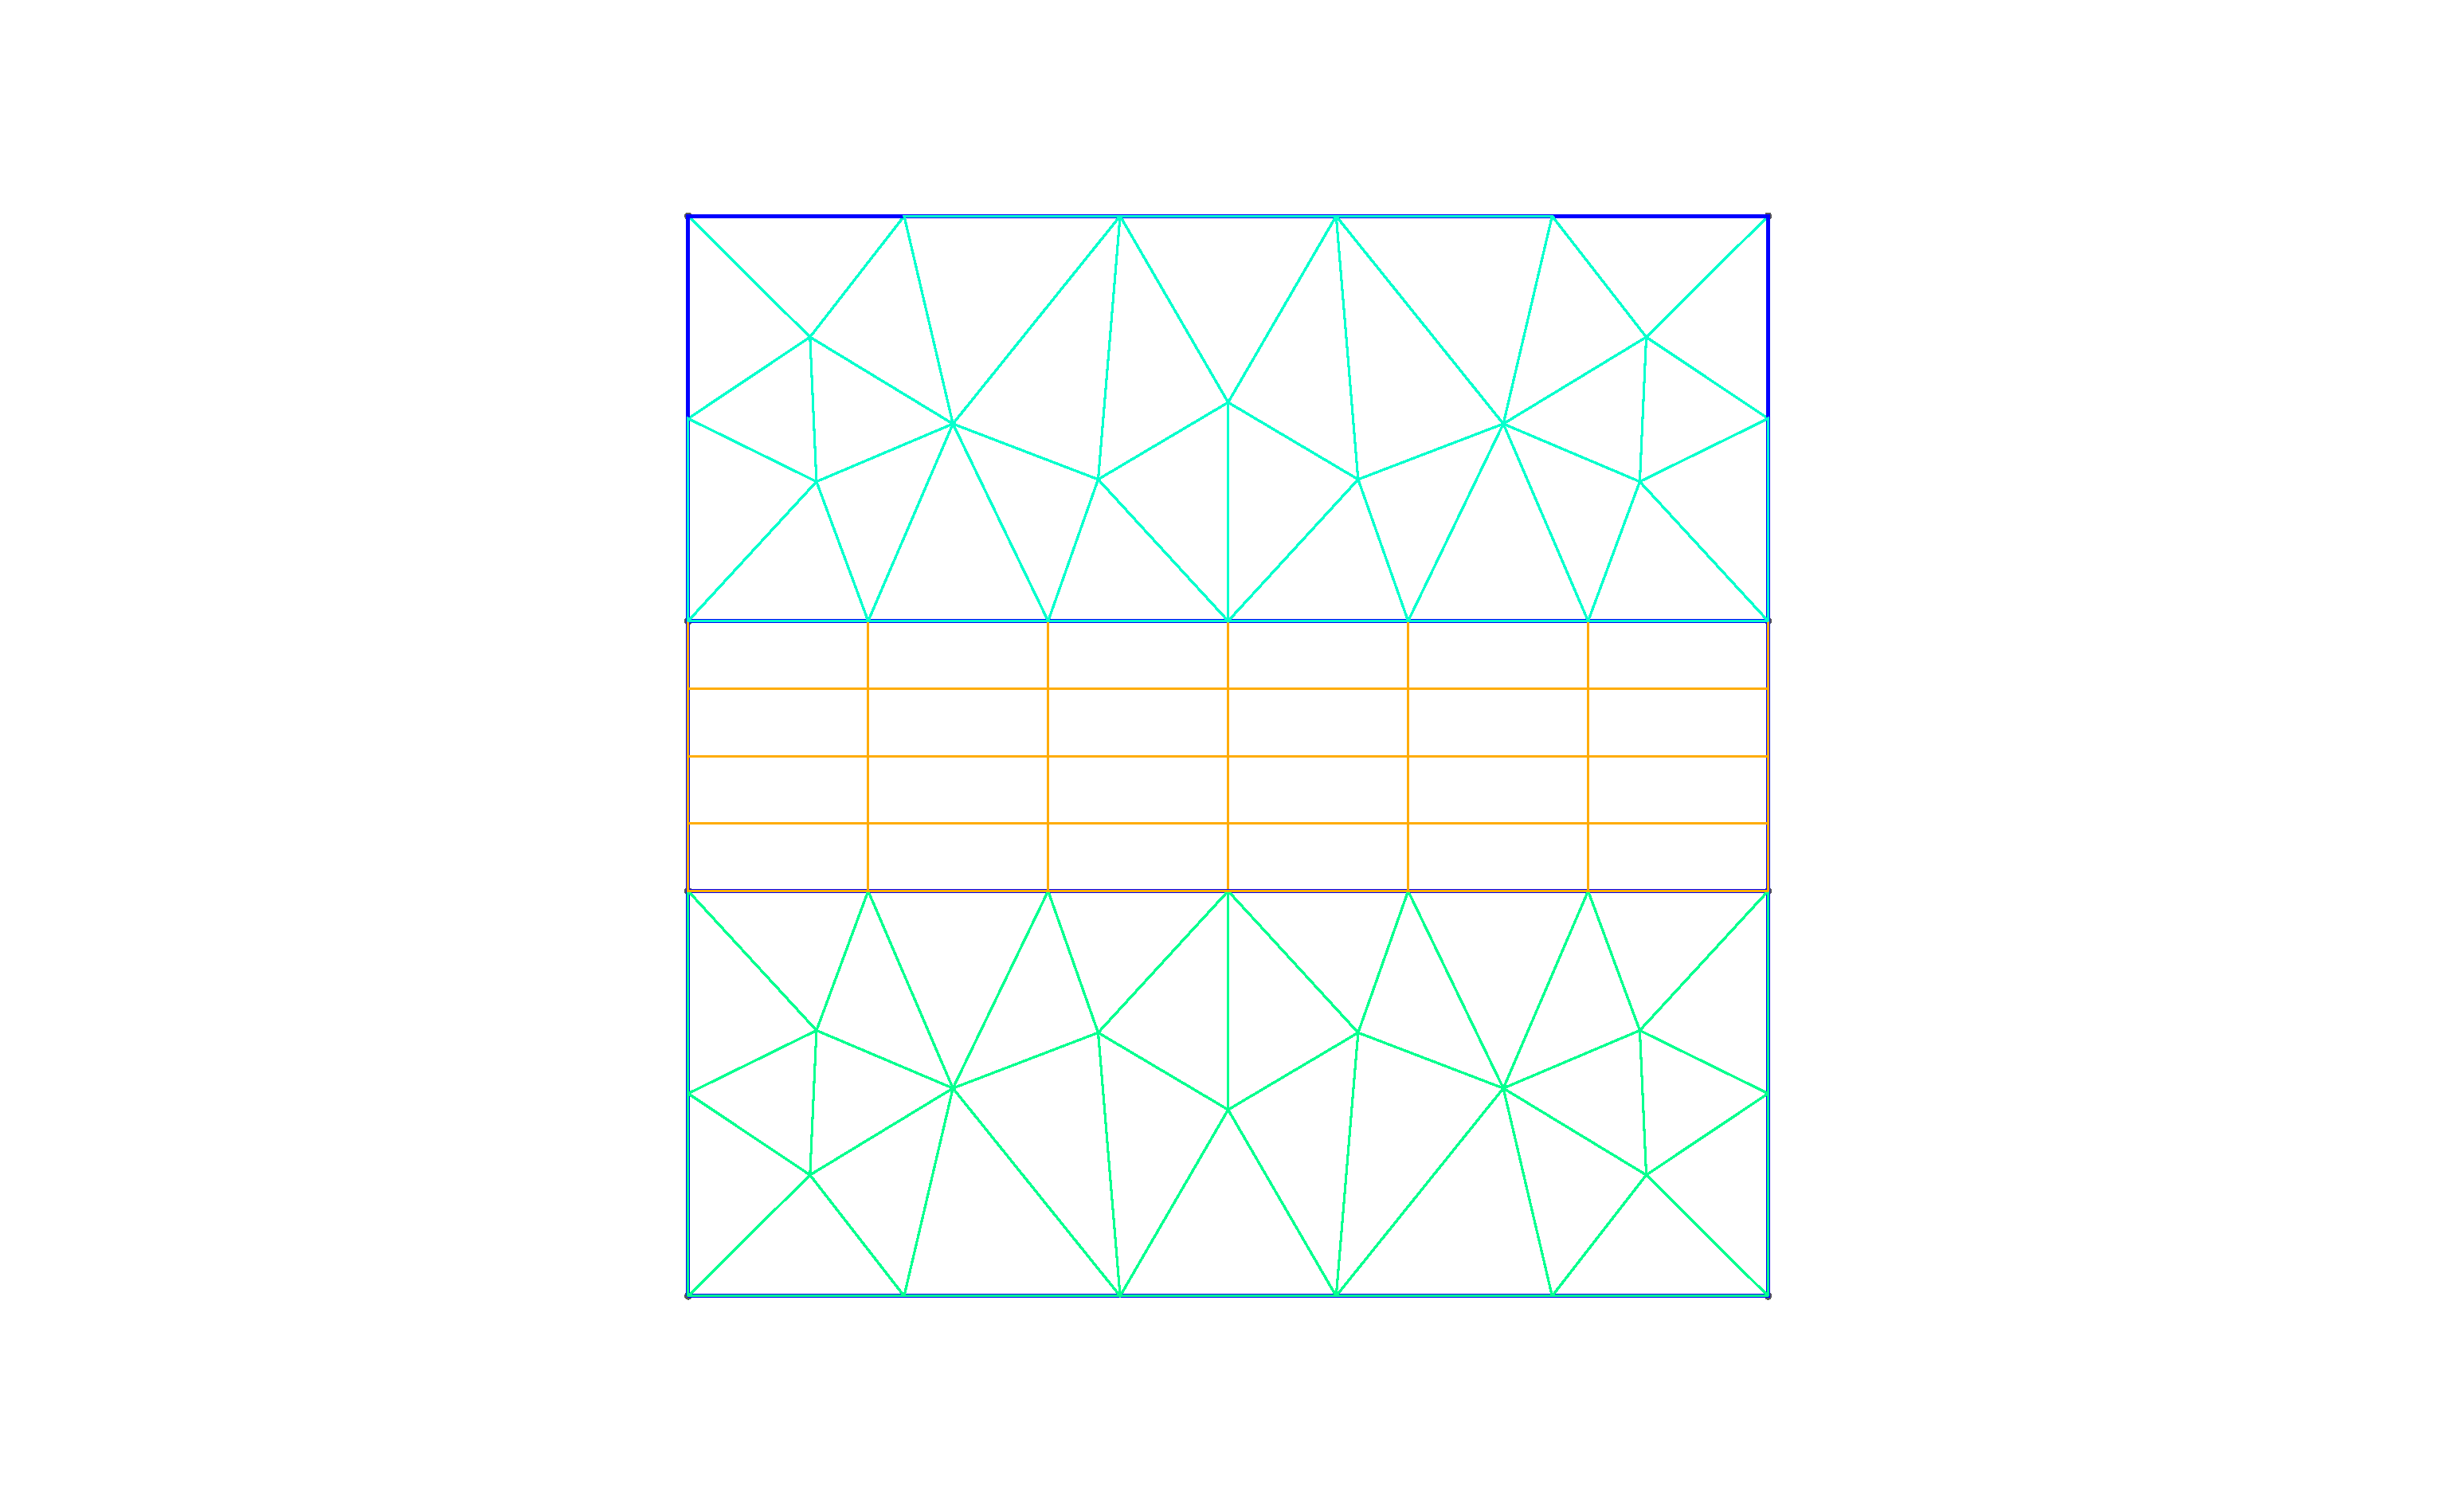
\includegraphics[width=5cm]{Figures/ADR_mesh_gmsh}
\caption{Mesh generated by Gmsh.}
\label{f:gmsh}
\end{center}
\end{figure}
%
It is now possible to visualise the Jacobian distribution across the mesh, \inlsh{ADR\_mesh.xml} 
by using the Nektar++ built-in post-processing routines
%
\begin{lstlisting}[style=BashInputStyle]
nektar++/builds/utilities/PostProcessing/XmlToVtk -j ADR_mesh.xml 
\end{lstlisting}
%
where the optional command -j calculate the Jacobian distribution for each element of the mesh.
This will produce a \inlsh{ADR\_mesh.vtu} file which can be directly read by the open-source 
visualisation tool called Paraview. In Fig. \ref{f:Jac} we show the Jacobian distribution for the 
mesh considered in this tutorial, \inlsh{ADR\_mesh.xml}.
%
\begin{figure}[h!]
\begin{center}
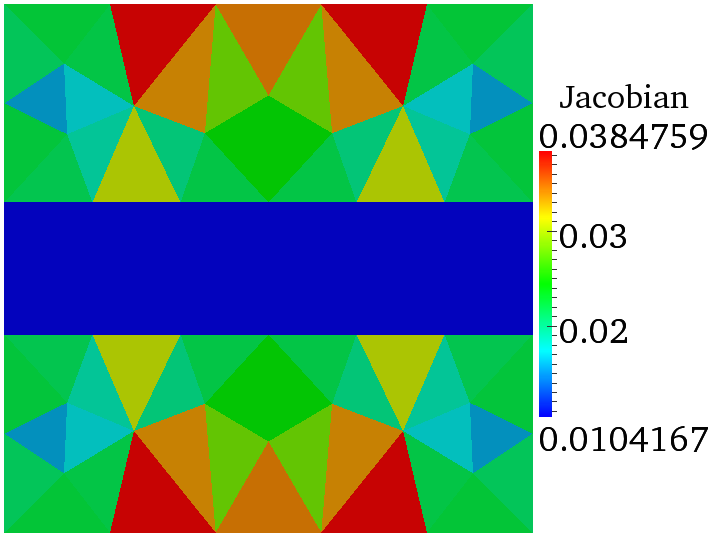
\includegraphics[width=6cm]{Figures/ADR_mesh_jacobian.png}
\caption{Jacobian distribution.}
\label{f:Jac}
\end{center}
\end{figure}
%
Before configuring the input files, if we want to use periodic boundary conditions, we 
need to make sure that the edges of the two periodic boundaries (i.e. $x_{b} = [-1, 1],
y_{b}$) are properly aligned. Gmsh and the \inltt{MeshConvert} routine within Nektar++ 
does not guarantee proper alignment. However, \inltt{MeshConvert} provides a module, 
namely \inltt{peralign}, that enforces the reordering of pair of edges (for more details 
refer to the User-Guide). We can apply this by using the following command:
%
\begin{lstlisting}[style=BashInputStyle]
nektar++/builds/utilities/PreProcessing/MeshConvert/MeshConvert \
-m peralign:surf1=200:surf2=400:dir=x ADR_mesh.xml ADR_mesh_aligned.xml
\end{lstlisting}
%
where \inltt{-m peralign} is selecting the module for aligning the edges which are 
specified by \inltt{surf1} and \inltt{surf2} (their IDs in this case are 200 and 400) 
and \inltt{dir} is the direction to which the two periodic edges are perpendicular 
to (in this case $x$).

After having typed the last command, we have a mesh, \inlsh{ADR\_mesh\_aligned.xml},
which is fully compatible with Nektar++ and which allows us applying periodic boundary 
conditions without encountering errors. 

We can therefore now configure the conditions: initial conditions, boundary conditions, 
parameters and solver settings. 

\section{Configuring the expansion bases and the conditions}
\label{adr-configuring}
For setting the various parameters and settings needed we create a new file 
called \inltt{ADR\_conditions.xml}, which can be found within the resources 
provided for this tutorial. 
This new file contains the \inltt{EXPANSIONS} tag where we can specify 
the polynomial order to be used inside each element of the mesh, the type 
of expansion bases and the type of points:
%
\begin{lstlisting}[style=XMLStyle]
<EXPANSIONS>
    <E COMPOSITE="C[1]" NUMMODES="5" TYPE="MODIFIED" FIELDS="u" />
    <E COMPOSITE="C[2]" NUMMODES="5" TYPE="MODIFIED" FIELDS="u" />
    <E COMPOSITE="C[3]" NUMMODES="5" TYPE="MODIFIED" FIELDS="u" />
</EXPANSIONS>
\end{lstlisting}
%
where \inltt{TYPE} allows selecting the basis functions, \inltt{NUMMODES} is the number 
of coefficients we want to use for the basis functions (that is commonly equal to P+1 where 
P is the polynomial order of the basis functions), \inltt{FIELDS} is the solution variable of 
our problem and \inltt{COMPOSITE} are the mesh regions created by Gmsh. For additional 
details on the \inltt{EXPANSIONS} tag refer to the User-Guide.

After having configured the expansion bases, we need to setup the parameter and the solver 
settings. These can be found under the \inltt{CONDITIONS} tag:
%
\begin{lstlisting}[style=XMLStyle]
<CONDITIONS>
    <PARAMETERS>
        <P> FinTime  		= 1.0               		</P>
        <P> TimeStep 		= 0.001             		</P>
        <P> NumSteps 		= FinTime/TimeStep </P>
        <P> IO_CheckSteps = 100               		</P>
        <P> IO_InfoSteps 	= 100               		</P>
        <P> advx 			= 2.0               		</P>
        <P> advy 			= 0.0               		</P>
        <P> k 			= 2*PI              		</P>
    </PARAMETERS>
        
    <SOLVERINFO>
        <I PROPERTY="EQTYPE"                		VALUE="UnsteadyAdvection"   		/>
        <I PROPERTY="Projection"            		VALUE="DisContinuous"       		/>
        <I PROPERTY="AdvectionType"      		VALUE="WeakDG"              		/>
        <I PROPERTY="UpwindType"           	VALUE="Upwind"              		/>
        <I PROPERTY="TimeIntegrationMethod" 	VALUE="ClassicalRungeKutta4"	/>
    </SOLVERINFO>
    ...
\end{lstlisting}
%
In the \inltt{PARAMETERS} tag, \inltt{FinTime} is the final physical time of the simulation, 
\inltt{TimeStep} is the time-step, \inltt{NumSteps} is the number of steps, \inltt{IO\_CheckSteps} 
is the step-interval when a output file is written, \inltt{IO\_InfoSteps} is the step-interval when 
some information about the simulation are printed to the screen, \inltt{advx} and \inltt{advy} 
are the advection velocities V$_{x}$ and V$_{y}$, respectively and \inltt{k} is the $\kappa$ 
parameter.

In the \inltt{SOLVERINFO} tag, \inltt{EQTYPE} is the type of equation to be solved, \inltt{Projection} 
is the spatial projection operator to be used, \inltt{AdvectionType} is the advection operator 
to be adopted, \inltt{UpwindType} is the numerical flux to be used at the element interfaces 
when a discontinuous projection is used, \inltt{TimeIntegrationMethod} allows selecting the 
time-integration scheme. For all the possible solver-setting options refer to the User-Guide.

After having setup the main parameters of our simulation under the tag \inlsh{PARAMETERS} 
and the solver settings under the tag \inlsh{SOLVERINFO}, we can finalise the \inlsh{CONDITIONS}
tag by specifying the boundary and initial conditions:
%
\begin{lstlisting}[style=XMLStyle]
    ...
    <VARIABLES>
        <V ID="0"> u </V>
    </VARIABLES>
        
    <BOUNDARYREGIONS>
        <B ID="0"> C[100] </B>
        <B ID="1"> C[200] </B>
        <B ID="2"> C[300] </B>
        <B ID="3"> C[400] </B>
    </BOUNDARYREGIONS>
        
    <BOUNDARYCONDITIONS>
        <REGION REF="0">
            <D VAR="u" USERDEFINEDTYPE="TimeDependent"
            VALUE="sin(k*(x-advx*t))*cos(k*(y-advy*t))" />
        </REGION>
        <REGION REF="1">
            <P VAR="u" VALUE="[3]" />
        </REGION>
        <REGION REF="2">
             <D VAR="u" USERDEFINEDTYPE="TimeDependent"
            VALUE="sin(k*(x-advx*t))*cos(k*(y-advy*t))" />
        </REGION>
        <REGION REF="3">
            <P VAR="u" VALUE="[1]" />
        </REGION>
    </BOUNDARYCONDITIONS>
        
    <FUNCTION NAME="InitialConditions">
        <E VAR="u"  VALUE="sin(k*x)*cos(k*y)" />
    </FUNCTION>
    
    <FUNCTION NAME="AdvectionVelocity">
        <E VAR="Vx" VALUE="advx" />
        <E VAR="Vy" VALUE="advy" />
    </FUNCTION>
        
    <FUNCTION NAME="ExactSolution">
        <E VAR="u"  VALUE="sin(k*(x-advx*t))*cos(k*(y-advy*t))" />
    </FUNCTION>
</CONDITIONS>
\end{lstlisting}
%
In the above piece of \inltt{.xml}, \inltt{VARIABLES} is a non-optional parameter that needs to be specified 
and indicates the solution variable, \inltt{BOUNDARYREGIONS} are the boundary regions as defined in 
Gmsh, \inltt{BOUNDARYCONDITIONS} are the boundary conditions associated to the various boundary 
regions specified in the \inltt{BOUNDARYREGIONS} tag, where the syntax \inltt{<D VAR="u"} corresponds 
to a \inltt{D}irichlet boundary condition for the variable \inltt{u}, while \inltt{<P VAR="u"} corresponds 
to \inltt{P}eriodic boundary conditions. For additional details on the various options possible in terms 
of boundary conditions refer to the User-Guide.
Finally, \inltt{<FUNCTION NAME="InitialConditions">} allows the specification of the initial conditions, 
\inltt{<FUNCTION NAME="AdvectionVelocity">} specifies the advection velocities and is a non-optional 
parameters for the unsteady advection equation and \inltt{<FUNCTION NAME="ExactSolution">} 
permits us to provide the exact solution, through which the L$_{2}$ and L$_{\infty}$ errors are computed.




\section{Running the solver}
\label{adr-running}
Now that we have the mesh file compatible with Nektar++ and periodic boundary conditoins, 
\inlsh{ADR\_mesh\_aligned.xml}, and we have completed the condition file, \inlsh{ADR\_conditions.xml}, 
we can run the solver by using the following command:
%
\begin{lstlisting}[style=BashInputStyle]
nektar++/builds/solvers/ADRSolver/ADRSolver \
    ADR_mesh_aligned.xml ADR_conditions.xml
\end{lstlisting}
%
Note that we have written the mesh in a separate file from the conditions. This is generally more efficient 
because it allows reopening just the condition file which is much smaller in size than the mesh file (especially 
for large problems). However, we could also have written both the mesh and the conditions in unique file and 
used the same command as above for running the solver (in this case with just one file instead of two as line 
argument).

As soon as the file finishes running, we should see the following screen output:
%
\begin{lstlisting}[style=BashInputStyle]
=========================================
	        EquationType: UnsteadyAdvection
	        Session Name: ADR_mesh_aligned
	        Spatial Dim.: 2
	  Max SEM Exp. Order: 5
	      Expansion Dim.: 2
	      Riemann Solver: Upwind
	      Advection Type: 
	     Projection Type: Discontinuous Galerkin
	           Advection: explicit
	           Diffusion: explicit
	           Time Step: 0.001
	        No. of Steps: 1000
	 Checkpoints (steps): 100
	    Integration Type: ClassicalRungeKutta4
==========================================
Initial Conditions:
  - Field u: sin(k*x)*cos(k*y)
Writing: "ADR_mesh_aligned_0.chk"
Steps: 100      Time: 0.1          CPU Time: 0.435392s
Writing: "ADR_mesh_aligned_1.chk"
Steps: 200      Time: 0.2          CPU Time: 0.430588s
Writing: "ADR_mesh_aligned_2.chk"
Steps: 300      Time: 0.3          CPU Time: 0.428503s
Writing: "ADR_mesh_aligned_3.chk"
Steps: 400      Time: 0.4          CPU Time: 0.428529s
Writing: "ADR_mesh_aligned_4.chk"
Steps: 500      Time: 0.5          CPU Time: 0.430142s
Writing: "ADR_mesh_aligned_5.chk"
Steps: 600      Time: 0.6          CPU Time: 0.429481s
Writing: "ADR_mesh_aligned_6.chk"
Steps: 700      Time: 0.7          CPU Time: 0.433232s
Writing: "ADR_mesh_aligned_7.chk"
Steps: 800      Time: 0.8          CPU Time: 0.431088s
Writing: "ADR_mesh_aligned_8.chk"
Steps: 900      Time: 0.9          CPU Time: 0.427919s
Writing: "ADR_mesh_aligned_9.chk"
Steps: 1000     Time: 1            CPU Time: 0.436098s
Writing: "ADR_mesh_aligned_10.chk"
Time-integration  : 4.31097s
Writing: "ADR_mesh_aligned.fld"
-------------------------------------------
Total Computation Time = 4s
-------------------------------------------
L 2 error (variable u) : 0.00863475
L inf error (variable u) : 0.0390366
\end{lstlisting}
%
where the L2 and L inf errors are evaluated against the \inltt{<FUNCTION NAME="ExactSolution">} 
provided in the \inlsh{ADR\_conditions.xml} file. To have a more detailed view on the solver settings
and parameters used, it is possible to use the \inltt{-v} option (which stands for verbose) as follows:
%
\begin{lstlisting}[style=BashInputStyle]
nektar++/builds/solvers/ADRSolver/ADRSolver -v \
    ADR_mesh_aligned.xml ADR_conditions.xml
\end{lstlisting}
%
The simulation has now produced 11 \inltt{.chk} binary files and a final \inltt{.fld} binary file (which 
in this case is identical to the tenth \inltt{.chk} file). These binary files contain the result of the simulation
every 100 time-steps. This output interval has been chosen through the parameter \inltt{IO\_CheckSteps} 
in \inlsh{ADR\_conditions.xml}, which was set equal to 100. Also, it is possible to note that every 100 
time-steps the solver outputs the physical time of the simulation and the CPU time required for doing 
100 time-steps. The interval of 100 time-steps is decided through the parameter \inltt{IO\_InfoSteps}, 
which was also equal to 100.


\section{Post-processing}
\label{adr-post}
Now that the simulation has been completed, we need to post-process the file in order to visualise 
the results. In order to do so, we can use the built-in post-processing routines within Nektar++.
In particular, we can use the following command
%
\begin{lstlisting}[style=BashInputStyle]
nektar++/builds/utilities/PostProcessing/FieldConvert ADR_mesh_aligned.xml \
    ADR_conditions.xml ADR_mesh_aligned_0.chk ADR_mesh_aligned_0.vtu
\end{lstlisting}
%
which generates a \inltt{.vtu} file that is a readable format for the open-source package Paraview.
We can now open the \inltt{.vtu} file just generated (which corresponds to the initial condition, being 
the number `0' \inltt{.chk} file) and visualise it with Paraview. This produces the image in Fig.~(\ref{f:IC}).
%
\begin{figure}[h!]
\centering
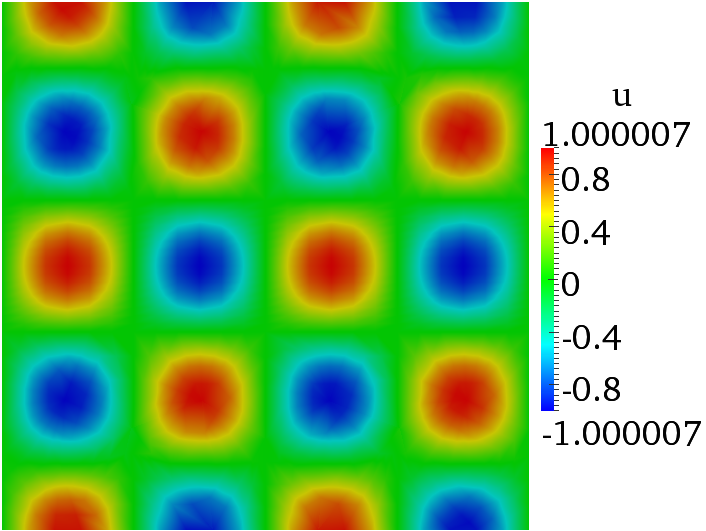
\includegraphics[width=0.4\textwidth]{Figures/ADR_mesh_IC}
\caption{Initial solution}
\label{f:IC}
\end{figure}~
%
It is possible to use the same post-processing command for visualising the other \inltt{.chk}, 
thus monitoring the evolution of the simulation in time.  


\section{Summary}
The user should be now familiar with the following topics:
\vspace{-0.5cm}
\begin{itemize}
\item Generate a simple mesh in Gmsh and convert it in a Nektar++-compatible format.
\item Visualise the Jacobian distribution across the mesh in Paraview.
\item Setup the initial and boundary conditions, the parameters and the solver settings.
\item Run the ADR solver.
\item Post-process the data in order to visualise results in Paraview.
\end{itemize}


\section{Exercises left to the user}
$\bullet$ Increase the polynomial order and plot the L$_{2}$ error vs. the polynomial order 
in a semilogarithmic scale. \\[1em]
$\bullet$ Change the projection operator for a fixed polynomial error and look at the error.\\[1em]
$\bullet$ Increase the time-step for a fixed polynomial order and look at the error.





